\documentclass{article}

\usepackage{polski}
\usepackage[margin=1in]{geometry}
\usepackage[parfill]{parskip}
\usepackage{amsmath}
\usepackage{graphicx}
\usepackage{caption}
\usepackage{siunitx}
\usepackage[table,xcdraw]{xcolor}
\usepackage{hyperref}
\usepackage[T1]{fontenc}
\usepackage{comment}
\usepackage{float}

\begin{document}

\begin{center}
\bgroup
\def\arraystretch{1.5}
\begin{tabular}{|c|c|c|c|c|c|}
	\hline
	EAIiIB & \multicolumn{2}{|c|}{\begin{tabular}{@{}c@{}}Stanisław Borowy \\ Maciej Bobrek \end{tabular}} & Rok II & Grupa 1 & Zespół 5 \\
	\hline
	\multicolumn{3}{|c|}{\begin{tabular}{c}Temat: \\Spektrometr optyczny \end{tabular}} & 
	\multicolumn{3}{|c|}{\begin{tabular}{c}Numer ćwiczenia: \\83 \end{tabular}} \\
	\hline
	\begin{tabular}{@{}c@{}}Data wykonania \\ 01.01.2023 \end{tabular} & \begin{tabular}{@{}c@{}}Data oddania \\ 02.01.2023 \end{tabular} & 
	\begin{tabular}{c}Zwrot do popr.\\\phantom{data} \end{tabular} & \begin{tabular}{c}Data oddania\\\phantom{data}\end{tabular} &
	\begin{tabular}{c}Data zaliczenia\\\phantom{data}\end{tabular} & \begin{tabular}{c}Ocena\\\phantom{ocena}\end{tabular} \\[4ex]
	\hline
\end{tabular}
\egroup
\end{center}

\section{Cel ćwiczenia}
Wyznaczenie długości fali widma liniowego par rtęci za pomocą spektrometru z siatką
dyfrakcyjną.

\section{Wprowadzenie teoretyczne}

Zgodnie z postulatem Bohra, przejściu atomu z wyższego poziomu
energetycznego $E_j$ na niższy poziom energetyczny $E_i$ towarzyszy
emisja fotonu o energii równej
\begin{align*}
    E_j - E_i = hf,
\end{align*}
gdzie $h$ jest stałą Plancka, a $f$ częstotliwością emitowanego fotonu.
Patrząc przez spektrometr z siatką dyfrakcyjną, zjawisko to objawia
się jako dyskretnie rozłożone wiązki światła o różnych kolorach (długościach fali). Rozłożenie to jest dane wzorem
\begin{align}
    \lambda = \frac{d\sin{\alpha}}{n},
    \label{eq:lambd}
\end{align}
gdzie $\alpha$ jest kątem, o który musimy obrócić obiektyw
spektrometru, aby nakierować go na badaną wiązkę, $n$ rzędem widma,
$\lambda$ długością fali wiązki, a $d$ odległością pomiędzy szczelinami
siatki dyfrakcyjnej. Badanie struktury poziomów energetycznych
atomu będzie polegało na obliczaniu długości fali z \eqref{eq:lambd}
dla wszystkich występujących wiązek światła.

\section{Aparatura}
Do wykonania ćwiczenia zespół użył 
\begin{enumerate}
    \item Luneta 
    \begin{enumerate}
     \item okular
     \item wskaźnik
     \item obiektyw
     \end{enumerate}
    \item Stolik
    \begin{enumerate}
     \item tarcza stolika ze skalą kątową
     \item siatka dyfrakcyjna
     \end{enumerate}
    \item Kolimator
    \begin{enumerate}
     \item soczewka
     \item szczelina
     \end{enumerate}
    \item Lampa Rtęciowa
\end{enumerate}
Na rysunku poniżej został umiesczony schemat spektrometru.
\begin{figure}[h!]
    \centering
    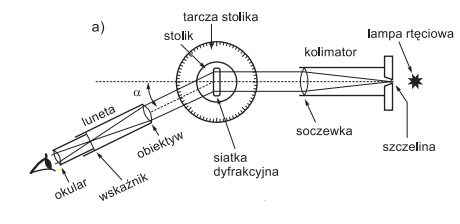
\includegraphics[scale=1]{cw83/spektrometr.png}
    \caption{Schemat spektrometru.}
\end{figure}
\section{Wyniki pomiarów}
Zespół na początku ustalił punkt odniesienia P, którym był prążek koloru białego koloru białego.
\begin{align*}
    P = 10'
\end{align*}
Następnie zespół przesuwając lunetą odczytywał wyniki ze skali kątowej dla wyraźnie widocznych prążków. Wyniki zebrano w tabeli \ref{tabela:1}
\begin{table}[h]
\centering
\begin{tabular}{|l|l|l|l|l|l|l|}
\hline
Kolor i rząd & Niebiesko-zielony & Zielony I   & Zielony II  & Żółty I     & Żółty II    & Czerwony    \\ \hline
Na (prawo)   & 16^\circ 58'           & 19^\circ 25'     & 41^\circ 34'     & 20^\circ 8'     & 43^\circ 30'    & 21^\circ 5'     \\ \hline
Na (lewo)    & 16^\circ 10'           & 18^\circ 34'     & 39^\circ 35'     & 19^\circ 15'     & 41^\circ 19'    & 20^\circ 9'     \\ \hline \\ \hline
Kolor i rząd    & Fioletowy I & Fioletowy II & Zielony I & Zielony II & Żółty I & Żołty II\\ \hline
Hg (prawo)     & 14^\circ 47'     & 31^\circ 02'      & 18^\circ 38'   & 39^\circ 35' & 19^\circ 42' & 19^\circ 48' \\ \hline
Hg (lewo)       & 14^\circ 20'     & 29^\circ 30'      & 17^\circ 47'   & 37^\circ 47'    & 19^\circ 50'&19^\circ 55' \\ \hline
\end{tabular}
\caption{Wyniki pomiarów kątów dla oznaczonych kolorów.}
\label{tabela:1}
\end{table}

\section{Opracowanie wyników pomiarów}
W obliczeniach będziemy stosować średnią kątów zmierzonych przekręcając
obiektyw w prawo i lewo. Dla każdego tak uśrednionego kąta obliczamy
długość fali $\lambda$ za pomocą \eqref{eq:lambd}.

Najpierw analizujemy wyniki dla atomu rtęci Hg.
\begin{table}[h]
\centering
\begin{tabular}{|l|l|l|l|l|l|}
\hline
Kolor i rząd    & Fioletowy I & Fioletowy II & Zielony I & Zielony II & Żółty \\ \hline
Hg (prawo)      & 14^\circ 47'     & 31^\circ 02'      & 18^\circ 38'   & 39^\circ 35'    & 19^\circ 45' \\ \hline
Hg (lewo)       & 14^\circ 20'     & 29^\circ 30'      & 17^\circ 47'   & 37^\circ 47'    & 19^\circ 52' \\ \hline
Hg (uśrednione) & 14^\circ 33' & 30^\circ 16'      & 18^\circ 13'   & 38^\circ 41'    & 19^\circ 49'  \\ \hline
$\lambda$ [nm] & 440.75 & 442.13 & 548.44 & 548.26 & 594.76 \\ \hline
\end{tabular}
\caption{Długości fal zaobserwowanych wiązek światła dla atomu rtęci Hg.}
\end{table}

Określenie błędu pomiaru długości fali $u(\lambda)$ 
jest bardzo trudne, gdyż wpływa na niego głównie błąd systematyczny 
wynikający z niedoskonałego wyjustowania przyrządu. Za szacunkową
wartość $u(\lambda)$ przyjmiemy różnicę wartości $\lambda$ zmierzoną
dla widm 1 i 2 rzędu (pomijając te widma, dla których została zmierzona
wartość tylko jednego rzędu). Dla atomu rtęci oznacza to
\begin{align*}
    u(\lambda) = \frac{(\lambda_{FII} - \lambda_{FI}) + (\lambda_{ZI} - \lambda_{ZII})}{2} \approx \SI{0.78}{nm}
\end{align*}

Analogicznie postępujemy dla atomu Na.

\begin{table}[h]
\begin{tabular}{|l|l|l|l|l|l|l|}
\hline
Kolor i rząd & Niebiesko-zielony & Zielony I   & Zielony II  & Żółty I     & Żółty II    & Czerwony    \\ \hline
Na (prawo)   & 16^\circ 58'           & 19^\circ 25'     & 41^\circ 34'     & 20^\circ 8'     & 43^\circ 30'    & 21^\circ 5'     \\ \hline
Na (lewo)    & 16^\circ 10'           & 18^\circ 34'     & 39^\circ 35'     & 19^\circ 15'     & 41^\circ 19'    & 20^\circ 9'     \\ \hline
Na           & 16^\circ 34'           & 19^\circ 00'     & 40^\circ 35'     & 19^\circ 42'     & 42^\circ 25'     & 20^\circ 37'     \\ \hline
$\lambda$ [nm]       & 500.23       & 571.17 & 570.66 & 591.40 & 591.68 & 617.74 \\ \hline
\end{tabular}
\end{table}

Natomiast niepewność pomiaru $u(\lambda)$ wynosi
\begin{align*}
    u(\lambda) = \frac{(\lambda_{ZI} - \lambda_{ZII}) + (\lambda_{ZoII} - \lambda_{ZoI})}{2} \approx \SI{0.40}{nm}
\end{align*}
Na podstawie wyliczonych długości fal możemy spróbować odszukać
przejścia odpowiadające zmierzonym liniom spektralnym i zapisać symbole początkowego
i końcowego poziomu energetycznego. Wyniki dla rtęci zebrano w tabeli
\begin{table}[h]
\centering
\begin{tabular}{|l|l|l|l|l|l|}
\hline
Kolor i rząd    & Fioletowy I & Fioletowy II & Zielony I & Zielony II & Żółty \\ \hline
$\lambda$ [nm] & 440.75 & 442.13 & 548.44 & 548.26 & 594.76 \\ \hline
Górny symbol Poz. Energ. &    7_3S_1   & 7_3S_1   &  7_3S_1    &  7_3S_1    & 6^1D_2                   \\ \hline
Dolny symbol  Poz. Energ. &     6^3P_1   &  6^3P_1   & 6^3P_2     & 6^3P_2    & 6^1P_1                   \\ \hline
                                    
\end{tabular}
\caption{Zmiana poziomów energetycznych dla rtęci}
\label{tab:przejscia}
\end{table}

\section{Wnioski}
Metodą rozszczepiania przez siatkę dyfrakcyjną udało nam się zbadać 
strukturę energetyczną atomu rtęci i sodu. 
\begin{itemize}
    \item Dla atomu rtęci znaleźliśmy przejścia odpowiadające długości fali
    \begin{itemize}
        \item Kolor fioletowy -- \SI{440.75}{nm}
        \item Kolor zielony -- \SI{548.44}{nm}
        \item Kolor żółty -- \SI{594.76}{nm}
    \end{itemize}
    Wyliczone długości zestawiliśmy ze znanymi przejściami zachodzącymi
    w atomie rtęci w tabeli \ref{tab:przejscia}.
    \item Dla atomu sodu znaleźliśmy przejścia odpowiadające długości fali
    \begin{itemize}
        \item Kolor niebiesko-zielony -- \SI{500.23}{nm}
        \item Kolor zielony -- \SI{571.17}{nm}
        \item Kolor żółty -- \SI{591.40}{nm}
        \item Kolor czerwony -- \SI{617.74}{nm}
    \end{itemize}
\end{itemize}
\end{document}